\section{Quotient Groups and Homomorphisms}

\subsection{Definitions and Examples}

\begin{note}[Set of Fibers as a Group]
    \begin{itemize}
        \item To study a group $G$, we will introduce the idea of a quotient group of $G$, which is essentially a ``smaller'' group from $G$ that we may use to study $G$ itself.
        \item The studying of this quotient group is equivalent to studying the homomorphisms of $G$. Recall that for a homomorphism $\phi : G \to H$, the \textit{fibers} of $\phi$ are the sets of elements of $G$ that project to a set of elements in $H$. We may present this pictorially as follows:
    \end{itemize}
    \begin{center}
        \begin{tikzpicture}
            \draw (0, 0) rectangle (10, 4);
            \node at (10.5, 2) {$G$};
            \node at (10.5, -2.5) {$H$};
            \draw (0, -2.5) -- (10, -2.5);

            \foreach \x in {1.5, 2.5, 5, 7.5, 8.5}
                \draw (\x, 0.5) -- (\x, 3.5);
                
            \foreach \x in {1.5, 2.5, 5, 7.5, 8.5}
                \draw[-{Latex[length=2mm]}] (\x, -0.5) -- (\x, -2);
                
            \foreach \x in {1.5, 2.5, 5, 7.5, 8.5}
                \fill (\x, -2.5) circle (2.5pt);
                
            \foreach \x in {3.75, 6.25}
                \node at (\x,2) {$\cdots$};

            \node at (5.5, -1.25) {$\phi$};
        \end{tikzpicture}
    \end{center}
    \begin{itemize}
        \item Two elements on the horizontal line in $H$ provides a natural idea of making the set of fibers into a group: Let $F_a$ be the fiber above $a$ and $F_b$ be the fiber above $b$, then $F_{ab}$ is the fiber above the product $ab$ so that $F_aF_b = F_{ab}$. Moreover, the identity of this group is $F_1 = \ker(\phi)$, associativity follows because of associativity in $H$, i.e., $(F_aF_b)F_c = F_{ab}F_c = F_{(ab)c} = F_{a(bc)} = F_aF_{bc} = F_a(F_bF_c)$. Lastly, the inverse of $F_a$ is simply $F_{a\inv}$. In general, the group $G$ has now been partitioned into pieces, and these pieces have formed into a quotient group.
    \end{itemize}
\end{note}

\begin{ex}[Example of Partitioning $\z$ Into $Z_n$]
    Define $\phi : \z \to Z_n$ by $\phi(a) = x^a$. Since $\phi(m + n) = x^{m + n} = x^mx^n = \phi(m)\phi(n)$, then $\phi$ is a group homomorphism. Moreover, $\phi$ is surjective. Then the fiber of $\phi$ over $x^a$ is the set
    \[\phi\inv(x^a) = \set{m \in \z \mid x^m = x^a} = \set{m \in \z \mid x^{m - a} = 1} = \set{m \in \z \mid \text{$n$ divides $m - a$}} = \set{m \in \z \mid m \equiv a \bmod n} = \bar  a\]
    the fibers of $\phi$ are precisely the residue classes modulo $n$. Then the above picture becomes
    \begin{center}
        \begin{tikzpicture}
            \draw (0, 0) rectangle (10, 4);
            \node at (10.5, 2) {$\z$};
            
            \draw (0, -2.5) -- (10, -2.5);
            \node at (10.5, -2.5) {$Z_n$};

            \node at (0.8, 2) {
            \begin{tabular}{c}
                $0$ \\
                $\pm n$ \\
                $\pm 2n$ \\
                $\pm 3n$ \\
                $\pm 4n$ \\
                $\vdots$
            \end{tabular}
            };
            \draw (1.6, 0) -- (1.6, 4);

            \node at (2.4, 2) {
            \begin{tabular}{c}
                $1$ \\
                $1 \pm n$ \\
                $1 \pm 2n$ \\
                $1 \pm 3n$ \\
                $1 \pm 4n$ \\
                $\vdots$
            \end{tabular}
            };
            \draw (3.2, 0) -- (3.2, 4);

            \node at (3.7, 2) {$\cdots$};
            \draw (4.2, 0) -- (4.2, 4);

            \node at (5.2, 2) {
            \begin{tabular}{c}
                $a$ \\
                $a \pm n$ \\
                $a \pm 2n$ \\
                $a \pm 3n$ \\
                $a \pm 4n$ \\
                $\vdots$
            \end{tabular}
            };
            \draw (6.2, 0) -- (6.2, 4);

            \node at (6.7, 2) {$\cdots$};
            \draw (7.2, 0) -- (7.2, 4);

            \node at (8.6, 2) {
            \begin{tabular}{c}
                $n - 1$ \\
                $(n - 1) \pm n$ \\
                $(n - 1) \pm 2n$ \\
                $(n - 1) \pm 3n$ \\
                $(n - 1) \pm 4n$ \\
                $\vdots$
            \end{tabular}
            };

            \foreach \x in {0.8, 2.4, 5.2, 8.6}
                \draw[-{Latex[length=2mm]}] (\x, -0.5) -- (\x, -2);

            \foreach \x in {0.8, 2.4, 5.2, 8.6}
                \fill (\x, -2.5) circle (2.5pt);

            \node at (0.8, -2.8) {$x^0 = 1$};
            \node at (2.4, -2.8) {$x^1$};
            \node at (5.2, -2.8) {$x^a$};
            \node at (8.6, -2.8) {$x^{n - 1}$};
        \end{tikzpicture}
    \end{center}
    In $Z_n$, we have $x^ax^b = x^{a + b}$ with corresponding fibers $\bar  a, \bar  b$, and $\bar{a + b}$, hence the corresponding group operation for the set of fibers is $\bar  a \cdot \bar  b = \bar{a + b}$, which is isomorphic to the group $\intmod \cong \im(Z_n)$. The identity is the multiples of $n$ in $\z$, or $n\z$. The remaining fibers are the translates $a + n\z$.
\end{ex}

\begin{defi}[Kernel]
    \label{defi3.1}
    Let $\phi : G \to H$ be a homomorphism. Then the \textbf{kernel} of $\phi$ is the set
    \[\ker(\phi) := \{g \in G \mid \phi(g) = 1\}\]
    where 1 is the identity of $H$.
\end{defi}

\begin{prop}[Homomorphism Properties]
    \label{prop3.1}
    \begin{enumerate}
        \item $\phi(1_G) = 1_H$, where $1_G$ and $1_H$ are the identities of $G$ and $H$, respectively.
        \item $\phi(g\inv) = \phi(g)\inv$ for every $g \in G$.
        \item $\phi(g^n) = \phi(g)^n$ for every $n \in \z$.
        \item $\ker(\phi) \leq G$.
        \item $\im(\phi) \leq H$.
    \end{enumerate}
    \begin{proofnum}
        \item $\phi(1_G) = \phi(1_G1_G) = \phi(1_G)\phi(1_G)$. By cancellation, $1_H = \phi(1_G)$.
        \item $1_H = \phi(1_G) = \phi(gg\inv) = \phi(g)\phi(g\inv)$ for all $g \in G$. Then $\phi(g)\inv = \phi(g\inv)$.
        \item This is true for $n = 0$, by part (1). It holds true for $n = 1$. Suppose it is true for any $n \in \zp$. Then
        \[\phi(g^{n + 1}) = \phi(g^ng) = \phi(g^n)\phi(g) = \phi(g)^n\phi(g) = \phi(g)^{n + 1}\]
        so the result for positive integers holds true by induction. Moreover, for any $n < 0$, then
        \[\phi(g^m) = \phi((g\inv)^{-m}) = (\phi(g)\inv)^{-m} = \phi(g)^m\]
        so it holds true for all $n \in \z$.
        \item Since $\phi(1_G) = 1_H$, then $\ker(\phi)$ is nonempty. Suppose $x, y \in \ker(\phi)$. Then $\phi(xy\inv) = \phi(x)\phi(y\inv) = 1_H1_H\inv = 1_H$ so that $xy\inv \in \ker(\phi)$. Then $\ker(\phi) \leq G$.
        \item Note that $\phi(1_G) = 1_H$ so that $1_H \in \im(\phi)$. Suppose $x, y \in \im(\phi)$. Then there exists $g, h \in G$ such that $\phi(g) = x$ and $\phi(h) = y$. Then $xy\inv = \phi(g)\phi(h\inv) = \phi(gh\inv)$. Since $gh\inv \in G$, then $xy\inv \in \im(\phi)$, hence $\im(\phi) \leq H$.
    \end{proofnum}
\end{prop}

\begin{defi}[Quotient Group]
    \label{defi3.2}
    \begin{itemize}
        \item Let $\phi : G \to H$ be a homomorphism with kernel $K$. Then the \textbf{quotient group}, or \textbf{factor group}, $G/K$ (read as $G$ \textit{modulo} $K$ or $G$ \textit{mod} $K$) is the group whose elements are the fibers of $\phi$ with group operation defined above: if $X$ is the fiber above $a$ and $Y$ is the fiber of $b$, then the product $XY$ is defined as the fiber above the product $ab$.
        \item This defines $K$ to be a single element in $G/K$ with the other elements of $G/K$ being translates of $K$. Then $G/K$ is collapsing the group $G$ by $K$
    \end{itemize}
\end{defi}

\begin{prop}[Defining Homomorphism Sets]
    \label{prop3.2}
    Let $\phi : G \to H$ be a homomorphism of groups with kernel $K$. Let $X \in G/K$ be the fiber above $a$, or $X = \phi\inv(a)$. Then
    \begin{enumerate}
        \item For any $x \in X$, $X = \{xk \mid k \in K\}$.
        \item For any $x \in X$, $X = \{kx \mid k \in K\}$.
    \end{enumerate}
    \begin{proofnum}
        \item Let $x \in X$ so that $\phi(x) = a$. Let
        \[xK = \{xk \mid k \in K\}\]
        For any $k \in K$, then
        \[\phi(xk) = \phi(x)\phi(k) = \phi(x) = a\]
        so that $xk \in X$, hence $xK \subseteq X$. Now suppose $y \in X$, and put $k = x\inv y$. Then
        \[\phi(k) = \phi(x\inv)\phi(y) = \phi(x)\inv\phi(y) = a\inv a = 1\]
        so that $k \in \ker(\phi)$. Since $k = x\inv y$, then $y = xk \in xK$ so that $X \leq xK$.
        \item The proof follows similarly as (1), where we define
        \[Kx = \{kx \mid k \in K\}\]
        Showing $Kx \subseteq X$ is similar, and if we set $k = yx\inv$, then $k \in \ker(\phi)$ so that $kx = y \in X$, hence $X \subseteq Kx$.
    \end{proofnum}
\end{prop}

\begin{defi}[Left and Right Cosets]
    \label{defi3.3}
    \begin{itemize}
        \item Let $N \leq G$ and $g \in G$. Then
        \[gN = \set{gn \mid n \in N} \text{ and } Ng = \set{ng \mid n \in N}\]
        are called the \textbf{left coset} and \textbf{right coset} of $N$ in $G$ respectively. Moreover, any element of a coset is a \textbf{representative} of that coset.
        \item If $N$ is the kernel of a homomorphism and $h$ is a representative for the coset $gN$ (or $Ng$), then $hN = gN$ (or $Nh = Ng$). This become for any subgroup $N$.
        \item In additive groups $G$, we write $g + N$ and $N + g$ for left and right cosets respectively. We may see that the left coset $gN$ is the left translate of $N$ by $g$ in $G$.
        \item \autoref{prop3.2} shows that the fibers of a homomorphisms are the left/right cosets of the kernel, i.e., the elements of the quotient group $G/K$ are the left cosets $gK$ for $g \in G$.
    \end{itemize}
\end{defi}

\begin{theo}[Coset Multiplication]
    \label{theo3.3}
    Let $G$ be a group with $K$ a group homomorphism from $G$ to another group. The set of left cosets of $K$ in $G$ defined with the operation
    \[uK \circ vK = (uv)K\]
    forms a group, $G/K$. In particular, this operation is well defined in that if $u' \in uK$ and $v' \in vK$, then $u'v' \in uvK$, and $u'v'K = uvK$. Moreover, this is also analogously defined for right cosets.
    \begin{proof}
        Let $X, Y \in G/K$ and let $Z = XY \in G/K$ so that $X, Y$, and $Z$ are left cosets of $K$. Since $K$ is the kernel of a group homomorphism, then $X = \phi\inv(a)$ and $Y = \phi\inv(b)$ for $a, b \in H$. Moreover, $Z = \phi\inv(ab)$ by definition. Let $x \in X$ and $y \in Y$ so that $\phi(x) = a$ and $\phi(y) = b$. Then $X = xK$ and $Y = yK$. Then
        \[\phi(u)\phi(v) = \phi(uv) = ab \iff uv \in \phi\inv(ab) \iff uv \in Z\]
        Then $Z$ is the left coset $uvK$. An exercise below will show that every $z \in Z$ is written as $xy$ for $x \in X$ and $y \in Y$. Then $XY = Z$, and by \autoref{prop3.2}, it follows that $xK = Kx$ and $yK = Ky$ for every $x, y \in G$.
    \end{proof}
\end{theo}

\begin{note}[Additional Coset Notes]
    \begin{itemize}
        \item By the preceding theorem, multiplication is independent of the particular representatives chosen. A coset $uK$ containing $u$ will usually be denoted with $\bar  u$, and a quotient group $G/K$ will be denoted as $\bar G$, and the product of two elements $\bar  u$ and $\bar  v$ is the coset containing $uv$, or $\bar{uv}$.
        \item The following is a pictorial representation of coset multiplication:
    \end{itemize}
    \begin{center}
        \begin{tikzpicture}
            \draw (0, 0) rectangle (10, 4);
            \node at (10.5, 2) {$G$};
            \draw (0, -2.5) -- (10, -2.5);
            \node at (10.5, -2.5) {$H$};

            \foreach \x in {1.6, 3.2, 5, 6.8, 8.4}
                \draw (\x, 0.5) -- (\x, 3.5);

            \fill (1.6, 3.3) circle (2pt);
            \node at (1.3, 3.3) {$u$};
            \fill (3.2, 0.7) circle (2pt);
            \node at (2.9, 0.7) {$v$};
            \fill (6.8, 2.7) circle (2pt);
            \node at (7.2, 2.7) {$uv$};
            
            \draw [dashed] (1.6, 3.3) to[bend left=10] (3.2, 0.7);
            \draw [dashed, -{Latex[length=2mm]}] (2.5, 2.1) to[bend left=25] (6.7, 2.7);
            
            \node at (4.1, 2) {$\cdots$};
            \node at (5.9, 2) {$\cdots$};

            \foreach \x in {1.6, 3.2, 6.8}
                \draw[-{Latex[length=2mm]}] (\x, -0.5) -- (\x, -1.8);

            \foreach \x in {1.6, 3.2, 6.8}
                \fill (\x, -2.5) circle (2.5pt);

            \node at (1.6, -2.8) {$a$};
            \node at (3.2, -2.8) {$b$};
            \node at (6.8, -2.8) {$ab$};

            \draw [dashed] (1.6, -2.5) edge[bend left=45] (3.2, -2.5);
            \draw [dashed, -{Latex[length=2mm]}] (2.6, -2.15) to[bend left=20] (6.7, -2.4);
        \end{tikzpicture}
    \end{center}
\end{note}

\begin{ex}[Quotient Group Examples]
    \begin{itemize}
        \item The homomorphism $\phi : \z \to Z_n$ has fibers $a + n\z$ of the kernel $n\z$. By \autoref{theo3.3}, the set of cosets forms a group under addition of representatives, which is $\intmod$.
        \item If $\phi : G \to H$ is an isomorphism, then $K = 1$ as $\phi$ is injective, and the fibers of $\phi$ are singleton subsets. It follows easily that $G/1 \cong G$ with the isomorphism $\psi : G/1 \to G$ given by $\psi(g1) = g$.
        \item The \textit{trivial homomorphism} is $\phi : G \to 1$ with $\ker(\phi) = G$ so that $G/G \cong Z_1 = \set 1$.
        \item Let $G = \r^2$ and $H = \r$. Define $\phi : \r^2 \to \r$ by $\phi((x, y)) = x$ so that $\phi$ is a projection onto the $x$-axis. This is clearly a homomorphism, as
        \[\phi((x, y) + (a, b)) = \phi((x + a, y + b)) = x + a = \phi(x, y) + \phi(a, b)\]
        Moreover,
        \[\ker(\phi) = \{(x, y) \mid \phi((x, y)) = 0\} = \{(x, y) \mid x = 0\}\]
        which is just the $y$-axis. Then the cosets in $\bar{{\r}^2}$ are the elements $\bar{(a, 0)}$ that represent
        \[(a, 0) + \text{$y$-axis}\]
        or left/right translates of the $y$-axis by some real number $a$ (hence the vertical line $x = a$). Note that the choice of representatives is not important, as any $y$-coordinate can be chosen without abandon. The group operation in $\bar{{\r}^2}$ is described as follows: in the perspective of the mapping $\phi$, then we can sum the lines $x = a$ and $x = b$ to obtain $x = a + b$, or if we add the coset representatives of the vertical line containing $(a, y)$ and the vertical line containing $(b, y')$, then we get the vertical line containing $(a + b, y + y')$. A diagram below describes this pictorially:
        \begin{center}
            \begin{tikzpicture}
                \draw (0, 0) rectangle (10, 4);
                \node at (10.5, 2) {$\r^2$};
                \draw [{Latex[length=2mm]}-{Latex[length=2mm]}] (0, -2.5) -- (10, -2.5);
                \node at (10.5, -2.5) {$\r$};

                \draw [dashed, -{Latex[length=2mm]}] (0.3, 2) -- (9.7, 2);
                \node at (9.8, 1.8) {$x$};

                \node at (2.2, 1.7) {$-1$};
                \node at (3.8, 1.7) {$0$};
                \node at (5.3, 1.7) {$1$};
                \node at (7.8, 1.7) {$a$};
                
                \draw [-{Latex[length=2mm]}] (4, 0.3) -- (4, 3.7);
                \node at (4.2, 3.7) {$y$};

                \foreach \x in {2.5, 5.5, 8}
                    \draw (\x, 0.3) -- (\x, 3.7);

                \foreach \x in {2.5, 4, 5.5, 8}
                    \draw [-{Latex[length=2mm]}] (\x, -0.3) -- (\x, -2.2);

                \node at (4.2, -1.2) {$\phi$};
                
                \foreach \x in {2.5, 4, 5.5, 8}
                    \fill (\x, -2.5) circle (2.5pt);

                \node at (2.5, -2.8) {$-1$};
                \node at (4, -2.8) {$0$};
                \node at (5.5, -2.8) {1};
                \node at (8, -2.8) {$a$};
            \end{tikzpicture}
        \end{center}
        \item Define $\phi : Q_8 \to V_4$ by
        \[\phi(\pm 1) = 1, \quad \phi(\pm i) = a, \quad \phi(\pm j) = b, \quad \phi(\pm k) = c\]
        To see that $\phi$ is a homomorphism, note the following:
        \begin{align*}
            \phi(ij) & = \phi(k) = c = ab = \phi(i)\phi(j) \\
            \phi(ik) & = \phi(j) = b = ac = \phi(i)\phi(k) \\
            \phi(jk) & = \phi(i) = a = bc = \phi(j)\phi(k)
        \end{align*}
        In each of these, we may note that we may swap the placements of the $a, b, c$ in the 3rd equality in each line as $V_4$ is abelian to get the corresponding negative $Q_8$ element. $\phi$ is surjective, and $\ker(\phi) = \set{\pm 1}$. We think of $\phi$ as an absolute value function, which collapses similar terms to just one value. The fibers of $\phi$ are $F_1 = \set{\pm 1}, F_a = \set{\pm i}, F_b = \set{\pm j}$, and $F_c = \set{\pm k}$, which subsequently collapse to $1, a, b,$ and $c$ respectively in $Q_8/\gen{-1}$. Moreover, note that the fibers are exactly equivalent to the cosets of $\ker(\phi)$ (for example, $F_a = i\ker(\phi) = \set{i, -i}$.
    \end{itemize}
\end{ex}

\begin{prop}[Set of Cosets Partition Group and Equivalency of Two Cosets]
    \label{prop3.4}
    Let $N$ be a subgroup of a group $G$. Then the set of left cosets of $N$ in $G$ form a partition of $G$. Moreover, for every $g, h \in G$, then $gN = hN$ if and only if $h\inv g \in N$. In particular, $gN = hN$ if and only if $g$ and $h$ are representatives of the same coset.
    \begin{proof}
        Since $N \leq G$, then $1 \in N$ so that $g \in gN$ for every $g \in G$. Then
        \[G = \bigcup_{g \in G} gN\]
        If $gN \cap hN$ is empty, then we are done. If it not, we then have some $k \in gN \cap hN$. Then $k = gn = hn'$ for some $n, n' \in N$. Then $g = kn\inv = hn'n\inv$, where we note that $n'n\inv \in N$ because $N \leq G$. Then for any $gn_0 \in gN$ for some $n_0 \in N$, we have $gn_0 = hn'n\inv n_0 \in hN$ so that $gN \subseteq hN$. A similar argument shows that $hN \subseteq gN$ so that they are equal, hence cosets are either distinct or are equal.
        
        From the preceding argument, we see that $gN = hN$ if and only if $g \in hN$ if and only if $g = hn$ for $n \in N$ if and only if $h\inv g \in N$. Moreover, $h \in gN$ implies that $h$ is a representative of $gN$ so that $hN = gN$ if and only if $g$ and $h$ represent the same coset.
    \end{proof}
\end{prop}

\begin{prop}[Coset Multiplication Part 2]
    \label{prop3.5}
    Let $G$ be a group with $N \leq G$.
    \begin{enumerate}
        \item The operation on the set of left cosets of $N$ in $G$ described by
        \[gN \cdot hN = (gh)N\]
        is well defined if and only if $xnx\inv \in N$ for every $x \in G$ and $n \in N$.
        \item If the above operation is well defined, then the set of left cosets of $N$ in $G$ forms a group. In particular, the identity of this group is the coset $1N = N$ and the inverse of $gN$ is $(gN)\inv = g\inv N$.
    \end{enumerate}
    \begin{proofnum}
        \item Suppose the operation is well defined, and let $g \in G$ and $n \in N$. Then $g\inv N = ng\inv N$. Since $1 \in N$, then $ng\inv 1 \in ng\inv N$ so that $ng\inv = g\inv n'$ for some $n' \in N$. Then $gng\inv \in N$.
        
        If $gng\inv \in N$ instead for every $g \in G$ and $n \in N$, suppose $g, g' \in gN$ and $h, h' \in hN$. Then
        \[g' = gn, \quad h' = hn' \quad \text{ for $n, n' \in N$}\]
        Then
        \[g'h' = (gn)(hn') = g(hh\inv)nhn' = gh(h\inv n(h\inv)\inv)n'\]
        where we note that $h\inv n(h\inv)\inv \in N$ by assumption. Then $g'h' \in ghN$ so that $g'h'N \cap ghN$ is nonempty. By \autoref{prop3.4}, then $g'h'N = ghN$.
        \item If the operation is indeed well defined, then the group axioms hold easily due to $G$ being a group. In particular, associativity holds as follows for any $g, h, k \in G$
        \[gN(hNkN) = gN(hkN) = g(hk)N = (gh)kN = (ghN)kN = (gNhN)kN\]
        The identity in $G/N$ is $1N$, and if $gNxN = 1N$ for $x \in G$, it follows that $gx = 1$ implies $x = g\inv$ so that $(gN)\inv= g\inv N$.
    \end{proofnum}
\end{prop}

\begin{defi}[Conjugate, Normal]
    \label{defi3.4}
    Let $G$ be a group with $g \in G$ and $N \leq G$.
    \begin{itemize}
        \item The element $gng\inv$ is the \textbf{conjugate} of $n \in N$ by $g$.
        \item The set $gNg\inv = \{gng\inv \mid n \in N\}$ is the \textbf{conjugate} of $N$ by $g$. Moreover, we say $g$ \textbf{normalizes} $N$ if $gNg\inv = N$.
        \item $N$ is called \textbf{normal} if every $g \in G$ normalizes $N$, or $gNg\inv = N$ for every $g \in G$. Moreover, we write $N \nsub G$.
    \end{itemize}
\end{defi}

\begin{theo}[Normal Subgroup Results]
    \label{theo3.6}
    Let $G$ be a group with $N \leq G$. Then the following are equivalent:
    \begin{enumerate}
        \item $N \nsub G$,
        \item $N_G(N) = G$,
        \item $gN = Ng$ for every $g \in G$,
        \item the operation on left cosets of $N$ in $G$ described in \autoref{prop3.5} makes the set of left cosets into a group,
        \item $gNg\inv \subseteq N$ for every $g \in G$.
    \end{enumerate}
    \begin{proof}
        $(1) \iff (2)$: $N \nsub G$ if and only if $gNg\inv = N$ for every $g \in G$ if and only if $N_G(N) = G$.
        
        $(2) \implies (3)$: Since $N_G(N) = G$, then $gNg\inv = N$ for every $g \in G$. In particular, $gng\inv = n'$ for $n, n' \in N$ so that $gn = n'g$, or $gN = Ng$.
        
        $(3) \implies (4)$: Since $gN = Ng$ for every $g \in G$, then $gn = n'g$ for some $n, n' \in N$, or that $gng\inv \in N$ for every $g \in G$. By \autoref{prop3.5}, the implication follows.
        
        $(4) \implies (5)$: The coset being formed into a group implies the operation is well defined, or that $gng\inv \in N$ for every $g \in G$. Then $gNg\inv \subseteq N$.

        $(5) \implies (1)$: If $gNg\inv \subseteq N$ for every $g \in G$, then $g\inv Ng \subseteq N$ in particular. Let $n \in N$. Then for some $g \in G$, we have that $gng\inv \in N$. Then $n = g(g\inv ng)g\inv \in gNg\inv$ so that $N \subseteq gNg\inv$, hence $N \nsub G$.
    \end{proof}
\end{theo}

\begin{note}[Calculating a Normal Subgroup]
    \begin{itemize}
        \item A good goal is to minimize the computations necessary to determine if $N \nsub G$. Particularly, we minimize the calculations of all conjugates $gng\inv$ for some $n \in N$ and $g \in G$.
        \item In a later exercise, it will suffice to note that the elements of $N$ normalize $N$ itself since $N \leq G$. Moreover, if $N$ is found to have a set of generators, then we may only check the generators, since the conjugate of a product is the product of its conjugates, and the conjugate of the inverse is the inverse of a conjugate.
        \item If a set of generators for $G$ is also known, then we may only check that these generators normalize $N$, so in particular, knowing both sets of generators for $G$ and $N$ reduces the calculations considerably.
        \item Some examples show that directly showing $N_G(N) = G$ proves that $N \nsub G$ without computing all conjugates.
    \end{itemize}
\end{note}

\begin{prop}[Subgroup is Normal If and Only If Kernel]
    \label{prop3.7}
    Let $G$ be a group with $N \leq G$. Then $N \nsub G$ if and only if $\ker(\phi) = N$ for some homomorphism $\phi$.
    \begin{proof}
        Suppose $N \nsub G$. Define the mapping $\pi : G \to G/N$ given by
        \[\pi(g) = gN, \quad \text{for every $g \in G$}\]
        Then $\pi$ is a homomorphism, because
        \[\pi(gh) = (gh)N = gNhN = \pi(g)\pi(h)\]
        Then
        \[\ker(\pi) = \{g \in G \mid \pi(g) = 1N = N\} = \{g \in G \mid gN = N\} = \{g \in G \mid g \in N\} = N\]
        so that $N$ is the kernel of a homomorphism. Conversely, if $N$ is the kernel instead, then \autoref{prop3.2} says that the left and right cosets of $N$ with both being the fibers of the homomorphism. Then \autoref{theo3.6} implies that $N \nsub G$.
    \end{proof}
\end{prop}

\begin{defi}[Natural Projection]
    \label{defi3.5}
    Let $N \nsub G$. The homomorphism $\pi : G \to G/N$ defined by $\pi(g) = gN$ is the \textbf{natural projection} of $G$ onto $G/N$. Moreover, if $\bar H \leq G/N$, then the \textbf{complete preimage} of $\bar G$ in $G$ is $\pi\inv(\bar H)$.
\end{defi}

\begin{note}[A Word on Normal Subgroups and Quotient Groups]
    \begin{itemize}
        \item We first note that the complete preimage of a subgroup of $G/N$ is a subgroup of $G$ that contains $N$ since they are the elements that map $\bar 1 \mapsto \bar H$.
        \item A criterion that determines a subgroup $N$ of $G$ is the kernel of a homomorphism is when
        \[N_G(N) = G\]
        Then the normalizer of a subgroup $N$ of $G$ determines ``how close'' $N$ is to being a normal subgroup of $G$, hence the choice of name. We note that being normal depends on the relation of $N$ to $G$ rather than depending on the structure of $N$ itself, i.e., it may be true that $N \nsub G$ but $N \not\nsub H$ for some $H \supseteq G$.
        \item The kernel of a homomorphism is a normal subgroup $N$ of $G$, and the quotient $G/N$ is naturally isomorphic to $\im(\phi(G))$. Conversely, for $N \nsub G$, then we are equipped with $G/N$ and $\pi : G \to G/N$ where $\ker(\pi) = N$ (the natural projection). It follows that when discussing homomorphic images of $G$ is equivalent to discussing quotient groups of $G$ and producing normal subgroups.
        \item Lastly, we emphasize that elements of a quotient group are subsets of $G$.
    \end{itemize}
\end{note}

\begin{ex}[Normal Subgroups and Associated Quotients]
    Let $G$ be a group.
    \begin{itemize}
        \item It is easy to show that $1 \nsub G$ and $G \nsub G$, and $G/1 \cong G$ and $G/G \cong 1$.
        \item If $G$ is abelian, then any $N \leq G$ is normal because for every $g \in G$ and $n \in N$, then
        \[gng\inv = gg\inv n = n \in N\]
        It must be that $G$ is abelian, not just $N$ being abelian.
        \item If $G = \z$, then every subgroup of $N$ is cyclic:
        \[N = \gen n = \gen{-n} = n\z, \quad \text{for some $n \in \z$}\]
        so that $G/N = \intmod$ is a cyclic group with generator $\bar 1 = 1 + n\z$. We also note that $\z = \gen 1$.
        \item Suppose $G = Z_k$, let $Z_k = \gen x$, and let $N \leq G$. Then $N = \gen{x^d}$ by \autoref{prop2.6}, where $d$ is the smallest power such that $x^d \in N$. Then
        \[G/N = \{gN \mid g \in G\} = \{x^\alpha N \mid \alpha \in \z\}\]
        By a following exercise that will show $x^\alpha N = (xN)^\alpha$, then $G/N = \gen{xN}$ so that the quotient group $G/N$ is cyclic with $xN$ as a generator. A following exercise will also show that $x^d \in N$ implies that $|xN| = d$. Moroever, \autoref{prop2.5} shows that $d = \abs G/ \abs N$. This discussion shows that \textit{quotient groups of a cyclic group are cyclic}, and if $G = \gen g$, then $G/N = \gen{\bar  g}$, where $\bar  g = gN$. If $G$ is finite in addition to being cyclic with $N \leq G$, then $|G/N| = \abs G/\abs N$.
        \item Suppose $N \leq Z(G)$. Then $N \nsub G$, since $gng\inv = n \in N$ for every $g \in G$ and $n \in N$. In particular, $Z(G) \nsub G$. Recall that $\gen{-1} \subseteq Q_8$ was seen to be the kernel of a homomorphism, but because $\gen{-1} = Z(Q_8)$, then we have another fashion of arguing for its normality in $Q_8$.
        \item Let $G = D_8$, and note that $Z(D_8) = \gen{r^2}$. Then for every $x \in D_8$, the coset $x\gen{r^2} = \{x, xr^2\}$. Since $D_8$ has 8 elements and $x\gen{r^2}$ has 2, there are 4 cosets consisting of two elements each in the quotient group:
        \[D_8/\gen{r^2} = \{\bar  1, \bar  r, \bar  s, \bar{rs}\}\]
        We then have that $D_8/\gen{r^2} \cong Z_4$ or $V_4$. However, we note the following:
        \begin{align*}
            (\bar  r)^2 & = r^2\gen{r^2} = 1\gen{r^2} = \bar  1 \\
            (\bar  s)^2 & = s^2\gen{r^2} = 1\gen{r^2} = \bar  1 \\
            (\bar{rs})^2 & = (rs)^2\gen{r^2} = 1\gen{r^2} = \bar  1
        \end{align*}
        so that every nonidentity element in the quotient group has order 2. Since no element has order 4, then $D_8/\gen{r^2}$ is not cyclic, hence $D_8/\gen{r^2} \cong V_4$.
    \end{itemize}
\end{ex}

\subsection{More on Cosets and Lagrange's Theorem}

\begin{theo}[Lagrange's Theorem]
    \label{theo3.8}
    Let $G$ be a finite group and let $H \leq G$. Then the order of $H$ divides the order of $G$, and the number of distinct left cosets of $H$ in $G$ is given by $\abs{G} / \abs{H}$.
    \begin{proof}
        Let $\abs H = n$ and let the number of left cosets of $H$ in $G$ be $k$. By \autoref{prop3.4}, the set of left cosets of $H$ in $G$ partition $G$. The mapping from $H \to gH$ defined by $h \mapsto gh$ is clearly a surjection, and is injective, since $gh_1 = gh_2$ implies $h_1 = h_2$ for $gh_1, gh_2 \in gH$. It follows that $\abs{gH} = \abs H = n$. Since $G$ is partitioned into $k$ disjoint subsets each with cardinality $n$, it follows that $\abs G = kn$ so that $k = \abs G/\abs H$.
    \end{proof}
\end{theo}

\begin{defi}[Index]
    \label{defi3.6}
    Let $G$ be a (possibly infinite) group with $H \leq G$. Then the number of left cosets of $H$ in $G$ is called the \textbf{index} of $H$ in $G$, denoted by $|G : H|$.
    \begin{itemize}
        \item If $G$ is finite, then $|G : H| = \abs G / \abs H$ by \autoref{theo3.8}.
        \item If $G$ is infinite, then $|G : H|$ may be finite or infinite. For example, $\set 0 \leq \z$ has infinite index, while $\gen n \leq \z$ has index $n$.
    \end{itemize}
\end{defi}

\begin{cor}[Order of Element Divides Group Order]
    \label{cor3.9}
    Let $G$ be a finite group and let $g \in G$. Then the order of $g$ divides the order of $G$. In particular, $g^{\abs G} = 1$.
    \begin{proof}
        \autoref{prop2.2} shows that $\abs g = \abs{\gen x}$. Then the first part follows by using Lagrange's Theorem on $H = \gen g$. Since $\abs G$ is a multiple of $\abs g$, the second part follows.
    \end{proof}
\end{cor}

\begin{cor}[Prime Order Implies Cyclic]
    \label{cor3.10}
    Let $G$ be a group with prime order $p$. Then $G$ is cyclic, and $G \cong Z_p$.
    \begin{proof}
        Let $g \in G$ be a nonidentity element. Then $\abs{\gen g} > 1$, and $\abs{\gen g} \mid p$ by \autoref{cor3.9}, hence $\abs{\gen g} = p$. It follows that $\gen g = G$, so that $G$ is cyclic. It follows that $G \cong Z_p$ by \autoref{theo2.4}.
    \end{proof}
\end{cor}

\begin{ex}[Normal Subgroup of $S_3$]
    Let $H = \gen{(1\ 2\ 3)}$ and $G = S_3$ so that $H \leq G$. Note that $H \leq N_G(H) \leq G$. Since $\abs H = 3$ and $\abs G = 6$, then $N_G(H)$ must either be 3 or 6. Observe that
    \[(1\ 2)(1\ 2\ 3)(1\ 2) = (1\ 3\ 2) = (1\ 2\ 3)\inv\]
    so that $(1\ 2) \in N_G(H)$, hence $N_G(H) \neq H$ so that $N_G(H) = G$. It follows that $H \nsub G$.
\end{ex}

\begin{ex}[Subgroups of Index 2 are Normal]
    Let $G$ be a group with $H \leq G$ such that $|G : H| = 2$. Pick $g \in G - H$ so that the two left cosets of $H$ in $G$ are $1H$ and $gH$. Since $1H = H$ and the cosets partition $G$, it must be that $gH = G - H$. A similar argument shows that $Hg = G - H$ so that $gH = Hg$. Then \autoref{theo3.6} shows that $H \nsub G$. By definition of index, then $|G/H| = 2$, and $G/H \cong Z_2$.

    We note this result is not because we may choose the same coset representatives 1 and $g$ for both the left and right cosets of $H$, but through a pigeon-hole principle: because $1H = H = H1$, then the index assumption shows the remaining elements to be the remaining coset, either left or right.
\end{ex}

\begin{note}[Transitivity of Normality]
    It is not generally true that if $N \nsub H$ and $H \nsub G$ then $N \nsub G$. For example, $\gen s \nsub \gen{s, r^2} \nsub D_8$, but $\gen s$ is not normal in $D_8$ because $rsr\inv = sr^2 \notin \gen s$.
\end{note}

\begin{ex}[Non-Normal Subgroup]
    Let $H = \gen{(1\ 2)} \leq S_3$. Since $H$ has prime index 3, then Lagrange's Theorem shows that $N_{S_3}(H)$ are either $H$ or $S_3$. Since $(1\ 3)(1\ 2)(1\ 3) = (2\ 3) \not\in H$, then $N_{S_3}(H) = H$, hence $H$ is not a normal subgroup of $S_3$.
    
    Another way to argue this is to consider the left and right cosets of $H$ in $S_3$. For example, $(1\ 3)H = \{(1\ 3), (1\ 2\ 3)\}$, while $H(1\ 3) = \{(1\ 3), (1\ 3\ 2)\}$. Since $(1\ 3)H$ is the unique left coset containing $(1\ 3)$, then $(1\ 3)H$ cannot be a left coset.

    Yet another way to see this is to observe that the multiplication of two cosets is not well-defined. For example, consider $1H$ and $(1\ 3)H$. Observe that $1H = (1\ 2)H$, yet $1(1\ 3) \neq (1\ 2)(1\ 3) = (1\ 3\ 2) \not\in H$ so that they are not elements of the same left coset. This shows that the cosets of a subgroup form a group \textit{only} when the subgroup is normal.
\end{ex}

\begin{ex}[Generalization of Previous Example]
    Let $G = S_n$ for $n \in \zp$, and fix $i \in \set{1, 2, \ldots, n}$. The stabilizer of $i$ is the set $G_i = \set{\sigma \in G \mid \sigma(i) = i}$. Now suppose $\tau \in G$ such that $\tau(i) = j$. Then $\tau\sigma(i) = j$ for all $\sigma \in G_i$. Moreover, if $\mu \in G$ such that $\mu(i) = j$, then $\tau\inv \mu(i) = i$ so that $\tau\inv\mu \in G_i$, hence $\mu \in \tau G_i$. Then the left coset $\tau G_i = \{\mu \in G \mid \mu(i) = j\}$ comprises of the permutations in $S_n$ that send $i$ to $j$. 

    It is clear that distinct left cosets have no elements in common, for otherwise if $\tau G_i = \pi G_i$ for $\tau, \pi \in G$ such that $\tau(i) = j$ and $\pi(i) = k$, then there would be some permutation $\mu \in \tau G_i$ such that $\mu(i) = k$ and $\mu(i) = j$, hence $\mu$ would not be well-defined. The number of distinct left cosets is precisely the number of images that $i$ may be sent to, namely $n$. It follows that $|G : G_i| = n$. 
    
    Note that elements of the left coset $\tau G_i$ are permutations that begin with $\sigma$ and end with $\tau$ so that $i \mapsto j$. It follows that elements of the right coset $G_i \tau$ are permutations that begin with $\tau$ and end with $\sigma$ so that $k \mapsto j$. Hence, if $k = \tau\inv(i)$, then $\tau(k) = i$, and $G_i\tau = \{\lambda \in G \mid \lambda(k) = i\}$. For $n > 2$ and $\tau \in G$, then $\tau G_i \neq G_i \tau$ in general, since there exists permutations that take $i$ to $j$ but do not take $k$ to $i$. Hence, $G_i$ is not a normal subgroup.
\end{ex}

\begin{note}[Converse of Lagrange's Theorem]
    \begin{itemize}
        \item Observe that the full converse of Lagrange's Theorem is not true, i.e., if $G$ is a finite group with $n$ dividing $\abs G$, then $G$ need not have a subgroup of order $n$. Consider $A$ to be the group of symmetries of a regular tetrahedron, where $\abs A = 12$. If $A$ had a subgroup $H$ of order 6, then $|A : H| = 2$ so that $H \nsub A$, and $A/H \cong Z_2$. It follows that the square of every element in $A/H$ is the identity, hence for every $g \in A$, then $(gH)^2 = 1H$ or that $g^2 \in H$. In particular, if $g \in A$ such that $\abs g = 3$, then $g^3H = gH = H$ so that $g \in H$, hence $H$ contains all elements of order 3. However, there are 8 elements of order 3 in $A$, which are the $120^\circ$ rotations about a line from a vertex to the center of the opposing face.
        \item Some partial converses to Lagrange's Theorem exists, namely that the full converse is true for finite \textit{abelian} groups. There are other theorems that guarantee the existence of subgroups of certain orders, such as Cauchy's Theorem and Sylow's Theorems.
    \end{itemize}
\end{note}

\begin{theo}[Cauchy's Theorem]
    \label{theo3.11}
    Let $G$ be a finite group with $p$ dividing $\abs G$. Then $G$ has an element of order $p$.
\end{theo}

\begin{theo}[Sylow]
    \label{theo3.12}
    Let $G$ be a finite group of order $p^\alpha m$, where $p$ is a prime with $p \nmid m$. Then $G$ has a subgroup of order $p^\alpha$.
\end{theo}

\begin{defi}[Product of Subgroups]
    \label{defi3.7}
    Let $H$ and $K$ be subgroups of a group $G$. Then their \textbf{product} is the set
    \[HK = \{hk \mid h \in H,\ k \in K\}\]
\end{defi}

\begin{prop}[Order of Subgroup Product]
    \label{prop3.13}
    Let $H$ and $K$ be finite subgroups of a group $G$. Then
    \[\abs{HK} = \frac{\abs H \abs K}{\abs{H \cap K}}\]
    \begin{proof}
        Note that $HK$ is a union of left cosets of $K$, namely
        \[HK = \bigcup_{h \in H} hK\]
        Since each coset of $K$ has $\abs K$ elements, we need to find the number of \textit{distinct} left cosets of the form $hK$ for $h \in H$. Observe that $h_1K = h_2K$ if and only if $h_2\inv h_1 \in K$ for $h_1, h_2 \in H$. Then $h_2\inv h_1 \in H \cap K$ if and only if $h_1(H \cap K) = h_2(H \cap K)$. Then the number of distinct left cosets of $K$ in $HK$ is equal to the number of distinct left cosets of $H \cap K$ in $H$, which is given by Lagrange's Theorem as $\abs H / \abs{H \cap K}$. Since each distinct cosets of $K$ contain $\abs K$ elements, then the formula follows.
    \end{proof}
\end{prop}

\begin{prop}[Product Subgroup Criterion]
    \label{prop3.14}
    Let $H$ and $K$ be subgroups of a group $G$. Then $HK \leq G$ if and only if $HK = KH$.
    \begin{proof}
        \rightimp Suppose $HK \leq G$. It is clear that $K \leq HK$ and $H \leq HK$ so that $KH \subseteq HK$. For the other containment, suppose $hk \in HK$ for $h \in H$ and $k \in K$. Since $HK \leq G$, there is some element $x \in HK$ such that $x\inv = hk$. Setting $x = h_0k_0$ for $h_0 \in H$ and $k_0 \in K$, we get that $hk = x\inv = k_0\inv h_0\inv \in KH$, hence $HK = KH$.

        \leftimp Suppose $HK = KH$, and observe that $1 \in HK$ so that it is nonempty. Let $x, y \in HK$, where $x = h_1k_1$ and $y = h_2k_2$ for $h_1, h_2 \in H$ and $k_1, k_2 \in K$. To show $xy\inv \in HK$, consider $xy\inv = h_1k_1k_2\inv h_2\inv$. Since $k_1k_2\inv h_2\inv \in KH = HK$, there exists $h_3 \in H$ and $k_3 \in K$ such that $h_3k_3 = k_1k_2\inv h_2\inv$ so that $xy\inv = h_1h_3k_3 \in HK$, hence $HK \leq G$.
    \end{proof}
\end{prop}

\begin{cor}[Normalizing Product Criterion]
    \label{cor3.15}
    Let $H$ and $K$ be subgroups of a group $G$ with $H \leq N_G(K)$. Then $HK \leq G$. In particular, if $K \nsub G$, then $HK \leq G$ for any $H \leq G$.
    \begin{proof}
        We prove that $HK = KH$ to utilize the preceding proposition. To that end, let $h \in H$ and $k \in K$. Since $K \nsub G$, then $hkh\inv \in K$, hence $hk = (hkh\inv)h \in KH$ so that $HK \subseteq KH$. Using a similar argument, we can see that $kh = h(h\inv kh) \in HK$ so that $KH \subseteq HK$, hence they are equal. By \autoref{prop3.14}, the corollary follows.
    \end{proof}
\end{cor}

\begin{ex}[Subgroup Product]
    \begin{itemize}
        \item If $HK = KH$, this does not imply elements of $H$ commute with $K$; rather, it implies that if $hk \in HK$, we may find corresponding $k' \in K$ and $h' \in K$ such that $hk = k'h'$, where $h$ need not be $h'$ nor $k$ be $k'$. For example, for $G = D_{2n}$ with $H = \gen r$ and $K = \gen s$, then $G = HK = KH$, but $rs \neq sr$.
        \item For some terminology, we say that $A$ \textit{normalizes} or \textit{centralizes} $K$ if $A \subseteq N_G(K)$ or $A \subseteq C_G(A)$ respectively. We may then rephrase \autoref{cor3.15} to say that $HK$ is a subgroup of $G$ when $H$ normalizes $K$, or if $K$ normalizes $H$.
        \item We show an example of using the order formula in \autoref{prop3.13} to prove that a finite group is a product of two of its subgroups. Let $G = S_4$, $H = D_8$, and $K = \gen{(1\ 2\ 3)}$, where $D_8$ is considered as a subgroup of $S_4$ by associating each symmetry with a permutation on 4 verticies. Explictly, these are the elements of $S_4$ that correspond to the elements of $D_8$:
        \[D_8 = \{1, (1\ 2\ 3\ 4), (1\ 3)(2\ 4), (1\ 4\ 3\ 2), (2\ 4), (1\ 2)(3\ 4), (1\ 3), (1\ 4)(2\ 3)\}\]
        where 1 is the top left vertex in a square then count clockwise. The first four elements are the rotations, while the others are reflections. In Exercise 3.2.8, we show that we may use Lagrange's Theorem to show $H \cap K = 1$, hence $|HK| = 24$ by \autoref{prop3.13}. Then $HK = S_4$ and since $HK$ is a group, then $HK = KH$. We quickly note that $H \nsubseteq K$ and $K \nsubseteq H$ so that we may not use \autoref{cor3.15} to conclude that $HK = KH$. 
    \end{itemize}
\end{ex}

\begin{note}[Equivalence of Studying Right Cosets]
    Lagrange's Theorem shows that in a finite group $G$, the number of left cosets of $H$ in $G$ equal the number of right cosets of $H$ in $G$, even though the left cosets are not right cosets in general. Some texts may denote $H \bl G$ to denote the set of right cosets of $H$ in $G$.
\end{note}

\subsection{The Isomorphism Theorems}

\begin{theo}[The First Isomorphism Theorem]
    \label{theo3.16}
    If $\phi : G \to H$ is a group homomorphism, then $\ker\phi \nsub G$ and $G/\ker\phi \cong \phi(G)$.
    \begin{proof}
        By \autoref{prop3.7}, we know that $\ker\phi \nsub G$. Let $K = \ker\phi$ and define the map $\psi : G/K \to \phi(G)$ by $\psi(gK) = \phi(g)$. Now suppose $gK = g'K$ for some $g, g' \in G$. It follows that $g\inv g' \in K$, hence $\phi(g\inv g') = 1$ which implies $\phi(g) = \phi(g')$ so that $\psi$ is well-defined. Moreover, 
        \[\psi(gKg'K) = \psi(gg'K) = \phi(gg') = \phi(g)\phi(g') = \psi(gK)\psi(g'K)\]
        so that $\psi$ is a homomorphism. It is also clear that $\psi$ is surjective, and since $gK = g'K$ if and only if $g\inv g' \in K$, then $\psi$ is injective. Therefore, $\psi$ is an isomorphism, and $G/K \cong \phi(G)$.
    \end{proof}
\end{theo}

\begin{cor}[Consequences of First Isomorphism Theorem]
    \label{cor3.17}
    Let $\phi : G \to H$ be a group homomorphism.
    \begin{enumerate}
        \item $\phi$ is injective if and only if $\ker\phi = 1$.
        \item $|G : \ker\phi| = |\phi(G)|$.
    \end{enumerate}
    \begin{proofnum}
        \item \rightimp If $\phi$ is injective, then $\phi(g) = 1$ implies $g = 1$, hence $\ker\phi = 1$.
        
        \noindent \leftimp $\ker\phi = 1$ implies $G/\ker\phi = G/1 \cong G$. By the First Isomorphism Theorem,$G \cong \phi(G)$ hence $\phi$ is injective.
        \item This follows directly from the First Isomorphism Theorem, since $|G : \ker\phi| = |G/\ker\phi| = |\phi(G)|$.
    \end{proofnum}
\end{cor}

\begin{theo}[The Second/Diamond Isomorphism Theorem]
    \label{theo3.18}
    Let $G$ be a group, let $A$ and $B$ be subgroups of $G$ and assume $A \leq N_G(B)$. Then $AB$ is a subgroup of $G$, $B \nsub AB$, $A \cap B \nsub A$ and $AB/B \cong A/A \cap B$.
    \begin{proof}
        \autoref{cor3.15} shows that $AB \leq G$. Because $A \leq N_G(B)$ and $B \leq N_G(B)$ trivially, then $AB \leq N_G(B)$ so that $B \nsub AB$.

        By normality of $B$ in $AB$, then $AB/B$ is well defined and we may define $\phi : A \to AB/B$ given by $\phi(a) = aB$. This is clearly a homomorphism, since $\phi = \pi|_A$, where $\pi : AB \to AB/B$ is the natural projection homomorphism. By definition, $\phi$ is surjective. Moreover, if $a \in \ker\phi$, then $aB = B$ so that $a \in B$, hence $a \cap B$. It follows that $\ker\phi = A \cap B$. By the First Isomorphism Theorem, then $A \cap B \nsub A$, and $A/A \cap B \cong AB/B$.
    \end{proof}
\end{theo}

\begin{note}[Further Discussion on the Diamond Isomorphism Theorem]
    Note that the theorem gives a new proof of the formula given in \autoref{prop3.13} when we have the case $A \leq N_G(B)$. Moreover, the theorem is called the Diamond Isomorphism because the involved subgroups of $G$ in the theorem make a diamond shape in the subgroup lattice. Note that $AB/A$ doesn't need to be a group, i.e., $A$ is not normal in $G$, but we still have $|AB: A| = |B : A \cap B|$. The diamond shape is shown below, where the the tick marks represent which quotient groups are isomorphic.
    \begin{center}
        \begin{tikzpicture}
            \node (G) at (0, 0) {$G$};
            \node (AB) at (0, -1) {$AB$};
            \node (A) at (-1, -2) {$A$};
            \node (B) at (1, -2) {$B$};
            \node (AcapB) at (0, -3) {$A \cap B$};
            \node (1) at (0, -4) {$1$};

            \node [rotate=-45] at (0.5, -1.5) {\scriptsize$|$};
            \node [rotate=-45] at (-0.5, -2.5) {\scriptsize$|$};

            \draw (G) -- (AB) -- (A) -- (AcapB) -- (1);
            \draw (AcapB) -- (B) -- (AB);
        \end{tikzpicture}
    \end{center}
\end{note}

\begin{theo}[The Third Isomorphism Theorem]
    \label{theo3.19}
    Let $G$ be a group and let $H$ and $K$ be normal subgroups of $G$ with $H \leq K$. Then $K/H \nsub G/H$ and
    \[ (G/H)/(K/H) \cong G/K \]
    Moreover, if we denote the quotient by $H$ with a bar, we may write this as
    \[ \bar G / \bar K \cong G/K \]
    \begin{proof}
        Let $gH \in G/H$, and consider $gHkHg\inv H \in gH(K/H)g\inv H$. That element is equal to $gkg\inv H$. Since $K \nsub G$, then $gkg\inv \in K$ so that $gkg\inv H \in K/H$, hence $gH(K/H)g\inv H \subseteq K/H$. By \autoref{theo3.6}, then $K/H \nsub G/H$.

        Define the map $\phi : G/H \to G/K$ given by $gH \mapsto gK$. To show $\phi$ is well defined, suppose $g_1H = g_2H$ for $g_1, g_2 \in G$. Then $g_1 = g_2h$ for some $h \in H$. Because $H \leq K$, then $h \in K$ so $g_1 = g_2h$ in $K$, hence $g_1K = g_2K$ or that $\phi(g_1H) = \phi(g_2H)$. Since our choice of $g$ is arbitrary, $\phi$ is a surjective homomorphism. Finally,
        \[\ker\phi = \set{gH \in G/H \mid \phi(gH) = 1K} = \set{gH \in G/H \mid gK = 1K} = \set{gH \in G/H \mid g \in K} = K/H\]
        so that by the First Isomorphism Theorem, then $(G/H)/(K/H) \cong G/K$.
    \end{proof}
\end{theo}

\begin{note}[A Remark on the Lattice Isomorphism Theorem]
    The following isomorphism theorem shows a relation between the lattice of subgroups of the quotient group $G/N$ and the lattice of subgroups of $G$. In particular, the lattice of subgroups for $G/N$ can be read from the lattice of subgroups of $G$ by collapsing the subgroup $N$ to the identity. More precisely, we may bijectively associate the subgroups of $G$ that contain $N$ with the subgroups of $G/N$ so that the lattice of $G/N$ appears in the lattice for $G$.
\end{note}

\begin{theo}[The Fourth/Lattice Isomorphism Theorem]
    \label{theo3.20}
    Let $G$ be a group with $N \nsub G$. Then there is a bijection from the set of subgroups $A$ of $G$ that contain $N$ onto the set of subgroups $\bar A$ of $G/N$. In particular, every subgroup of $\bar G$ is of the form $A/N$ for some subgroup $A$ of $G$ containing $N$ (its preimage in $G$ under the natural projection homomorphism from $G$ to $G/N$). This bijection has the following properties: for every $A, B \leq G$ with $N \leq A$ and $N \leq B$,
    \begin{enumerate}
        \item $A \leq B$ if and only if $\bar A \leq \bar B$,
        \item if $A \leq B$ , then $|B : A| = |\bar B : \bar A|$,
        \item $\bar{\gen{A, B}} = \gen{\bar A, \bar B}$,
        \item $\bar{A \cap B} = \bar A \cap \bar B$,
        \item $A \nsub G$ if and only if $\bar A \nsub \bar G$.
    \end{enumerate}
    \begin{proof}
        Let $\ac = \set{A \leq G \mid N \subseteq A}$ and $\bar{\ac} = \set{\bar A \leq \bar G}$. Define the map $\phi : \ac \to \bar{\ac}$ by $\phi(A) = \bar A = A/N$. Note that $\phi(A) \leq \bar G$ as follows: since $\bar 1 \in \bar A$, then $\bar A$ is nonempty. Moreover, for any $\bar a, \bar b \in \bar A$ where $a, b \in A$, then $ab\inv \in A$ implies $\bar a \bar b\inv = \overline{ab\inv} \in \bar A$, hence $\bar A \leq \bar G$. This also implies that $\phi$ is surjective, since for any $\bar A \in \bar{\ac}$, we know that the preimage of $\bar A$ under the natural projection homomorphism from $G$ to $G/N$ is some subgroup $A$ of $G$ containing $N$ such that $\phi(A) = \bar A$. Lastly, suppose $\phi(A) = \phi(B)$ for some $A, B \in \ac$. Then $\bar A = \bar B$ implies that for some $a \in A$, there is some $b \in B$ such that $\bar a = \bar b$, hence $aN = bN$ so that $b\inv a \in N \subseteq B$. It follows that $a = b(b\inv a) \in B$, hence $A \subseteq B$. A similar argument shows that $B \subseteq A$, hence $A = B$ so that $\phi$ is injective. Therefore, $\phi$ is a bijection.
        \begin{enumerate}
            \item \rightimp Suppose $A \leq B$ for $A, B \in \ac$, and suppose $\bar a \in \bar A$ for some $a \in A$. Since $A \leq B$, then $a \in B$ so that $\bar a \in \bar B$, hence $\bar A \leq \bar B$.
            
            \noindent \leftimp Suppose $\bar A \leq \bar B$ for $A, B \in \ac$, and suppose $a \in A$ for some $a \in A$. Then $\bar a \in \bar A$ so that $\bar a \in \bar B$, hence there is some $b \in B$ such that $\bar a = \bar b$. It follows that $aN = bN$ so that $b\inv a \in N \subseteq B$, hence $a = b(b\inv a) \in B$. Therefore, $A \leq B$.
            \item Consider a mapping $\psi : B/A \to \bar B / \bar A$ given by $\psi(bA) = \bar b \bar A$ for $b \in B$. To show $\psi$ is well-defined, suppose $b_1A = b_2A$ for some $b_1, b_2 \in B$. Then $b_2\inv b_1 \in A$, hence $\overline{b_2\inv b_1} \in \bar A$ so that $\bar b_1 \bar A = \bar b_2 \bar A$, hence $\psi(b_1A) = \psi(b_2A)$. It is clear that $\psi$ is a homomorphism, and it is surjective since for any $\bar b \bar A \in \bar B / \bar A$, there is some $b \in B$ such that $\psi(bA) = \bar b \bar A$. Finally, if $bA \in \ker\psi$, then $\psi(bA) = \bar A$ so that $\bar b \in \bar A$, hence $bN \in A/N$ or that $b \in A$. It follows that $\ker\psi = A/A = 1$, hence $\psi$ is an isomorphism. Therefore, $|B : A| = |B/A| = |\bar B / \bar A| = |\bar B : \bar A|$.
            \item $\bar x \in \bar{\gen{A, B}}$ if and only if $x = x_1x_2 \ldots x_n$ where $x_i \in A \cup B$ for each $1 \leq i \leq n$ if and only if $\bar x = \bar{x_1x_2} \ldots \bar{x_n}$ where $\bar{x_i} \in \bar A \cup \bar B$ for each $1 \leq i \leq n$ if and only if $\bar x \in \gen{\bar A, \bar B}$, hence $\bar{\gen{A, B}} = \gen{\bar A, \bar B}$.
            \item $\bar x \in \bar{A \cap B}$ if and only if $x \in A \cap B$ if and only if $x \in A$ and $x \in B$ if and only if $\bar x \in \bar A$ and $\bar x \in \bar B$ if and only if $\bar x \in \bar A \cap \bar B$, hence $\bar{A \cap B} = \bar A \cap \bar B$.
            \item \rightimp Suppose $A \nsub G$, and let $gN \in \bar G$. Then for any $\bar a \in \bar A$ where $a \in A$, we have that $gag\inv \in A$ so that $gNg\inv = gag\inv N \in \bar A$, hence $\bar A \nsub \bar G$.
            
            \noindent \leftimp Suppose $\bar A \nsub \bar G$, and let $g \in G$. Then for any $a \in A$, we have that $\bar g \bar a \bar g\inv \in \bar A$ so that $gag\inv N \in A/N$, hence $gag\inv \in A$, thus $A \nsub G$.
        \end{enumerate}
    \end{proof}
\end{theo}

\begin{ex}[Fourth Isomorphism Theorem Applied]
    \begin{itemize}
        \item Consider $G = Q_8$ with $N = \gen{-1}$. The isomorphic copy of $G/N$ consists of the double lines in the lattice of $G$ below. We have previously seen that $Q_8/\gen{-1} \cong V_4$ and the two lattices do indeed coincide.
        \begin{center}
            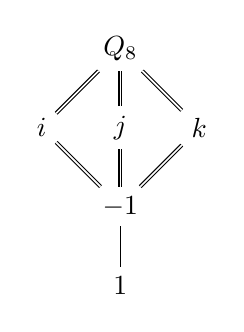
\begin{tikzpicture}
                \node (q8) at (0, 0) {$Q_8$};
                \node (i) at (-1, -1) {$\gen i$};
                \node (j) at (0, -1) {$\gen j$};
                \node (k) at (1, -1) {$\gen k$};
                \node (-1) at (0, -2) {$\gen{-1}$};
                \node (1) at (0, -3) {1};

                \draw (1) -- (-1);
                \draw [double] (-1) -- (i) -- (q8);
                \draw [double] (-1) -- (j) -- (q8);
                \draw [double] (-1) -- (k) -- (q8);
            \end{tikzpicture}
        \end{center}
        \item The same process gives the lattice of $D_8/\gen{r^2}$ in the lattice of $D_8$:
        \begin{center}
            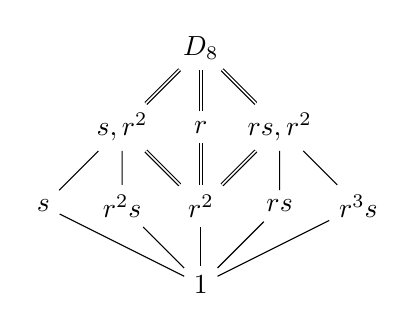
\begin{tikzpicture}
                \node (d8) at (0, 0) {$D_8$};
                \node (sr2) at (-1, -1) {$\gen{s, r^2}$};
                \node (r) at (0, -1) {$\gen r$};
                \node (rsr2) at (1, -1) {$\gen{rs, r^2}$};
                \node (s) at (-2, -2) {$\gen s$};
                \node (r2s) at (-1, -2) {$\gen{r^2s}$};
                \node (r2) at (0, -2) {$\gen{r^2}$};
                \node (rs) at (1, -2) {$\gen{rs}$};
                \node (r3s) at (2, -2) {$\gen{r^3s}$};
                \node (1) at (0, -3) {1};

                \draw (1) -- (s) -- (sr2);
                \draw (1) -- (r2s) -- (sr2);
                \draw (1) -- (r2);
                \draw [double] (r2) -- (sr2) -- (d8);
                \draw (1) -- (rs) -- (rsr2);
                \draw (1) -- (r3s) -- (rsr2);
                \draw [double] (r2) -- (r) -- (d8);
                \draw [double] (r2) -- (rsr2) -- (d8);
            \end{tikzpicture}
        \end{center}
    \end{itemize}
\end{ex}

\begin{note}[Further Discussion on the Lattice Isomorphism Theorem]
    \begin{itemize}
        \item Note that in the second example of $G = D_8$ with $N = \gen{r^2}$, there are subgroups of $G$ that do not correspond to the subgroups of $G/N$, such as $\gen r$. These subgroups are precisely those that do not contain $N$. In general, subgroups of $G$ point to the same subgroup in $G/N$.
        \item The image of a subgroup $H$ of $G$ under the natural projection homomorphism from $G$ to $G/N$ is the same as the image of the subgroup $HN$ of $G$, and $HN$ of $G$ contains $N$. Conversely, we see that the preimage of a subgroup $\bar H$ of $G/N$ contains $N$ and is the unique subgroup of $G$ containing $N$ whose image is $\bar H$ in $G/N$. In particular, it is the subgroups of $G$ containing $N$ which appear in the lattice for $G/N$.
        \item The two lattices above illustrate that the isomorphism type of a group cannot be determined by the isomorphism types of $G/N$ and $N$. For example, both $Q_8$ and $D_8$ have normal subgroups isomorphic to $Z_2$ with corresponding quotient groups isomorphic to $V_4$, yet $Q_8$ is not isomorphic to $D_8$.
        \item In a subgroup lattice, we may label the edges traced out between the subgroups with an integer $n$ such that $|A : B| = n$. Moreover, this integer is unchanged even with the subgroup lattice of the quotient groups by \autoref{theo3.20}(2).
    \end{itemize}
\end{note}

\begin{note}[Remark on Group Homomorphisms on Quotient Groups]
    There have been situations in the proofs of the isomorphism theorems that a homomorphism defined on $G/N$ is specified by giving the value of $\phi$ on the coset $gN$ in terms of $g$ alone. These situations required us showing that $\phi$ was well-defined, i.e., independent of the choice of $g$. We are actually defining a homomorphism $\Phi$ on $G$ itself by specifying the value of $\phi$ at $g$, hence independence of the choice of $g$ requires that $\Phi$ be trivial on $N$, i.e.,
    \[\text{$\phi$ is well defined on $G/N$ if and only if $N \leq \ker\Phi$.}\]
    We may check that a homomorphism on $G/N$ is well-defined by defining a homomorphism on $G$ and check that $N$ is contained in its kernel. We then say that $\Phi$ \textit{factors through} $N$, and $\phi$ is the \textit{induced} homomorphism on $G/N$. We may show this pictorially as follows:
    \begin{center}
        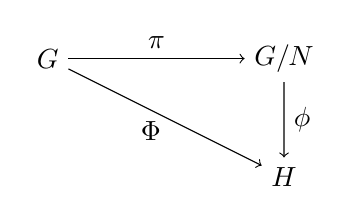
\begin{tikzpicture}[scale=1.5]
            \node (G) at (0,0) {$G$};
            \node (GN) at (2, 0) {$G/N$};
            \node (H) at (2, -1) {$H$};

            \draw[->] (G) -- (GN) node [midway, above] {$\pi$};
            \draw[->] (G) -- (H) node [midway, below left=-2pt] {$\Phi$};
            \draw[->] (GN) -- (H) node [midway, right] {$\phi$};
        \end{tikzpicture}
    \end{center}
    The diagram indicates that $\Phi = \phi \circ \pi$, i.e., the image in $H$ of an element in $G$ does not depend on the path taken in the dagram. We say that this diagram \textit{commutes}.
\end{note}